\documentclass[onecolumn]{article}

% Use the following line for the initial blind version submitted for review:
\usepackage{icml2020}

% If accepted, instead use the following line for the camera-ready submission:
%\usepackage[accepted]{icml2020}

\usepackage{natbib}

\usepackage[utf8]{inputenc} % allow utf-8 input
\usepackage[T1]{fontenc}    % use 8-bit T1 fonts
\usepackage{hyperref}       % hyperlinks
% Attempt to make hyperref and algorithmic work together better:
\newcommand{\theHalgorithm}{\arabic{algorithm}}

\usepackage{url}            % simple URL typesetting
\usepackage{booktabs}       % professional-quality tables
\usepackage{amsfonts}       % blackboard math symbols
\usepackage{nicefrac}       % compact symbols for 1/2, etc.
\usepackage{microtype}      % microtypography
\usepackage{multirow}				% for multi-row labels
\usepackage{subfig}					% for laying out multi-panel figures and tables 
\usepackage{cancel}					% for crossing out characters
\usepackage{amsmath}				% for splitting multi-line equations
\usepackage{placeins}				% for table and figure positioning
\usepackage{mathtools}			% for \vdotswithin{}
\usepackage{resizegather}   % for gathering multi-lines to one line
%packages for graph layout
\usepackage{graphicx}
\usepackage[pdf]{graphviz}
%format section headings compactly
\usepackage[compact]{titlesec}
\titlespacing{\section}{0pt}{2ex}{1ex}
\titlespacing{\subsection}{0pt}{1ex}{0ex}
\titlespacing{\subsubsection}{0pt}{0.5ex}{0ex}

\setlength{\textfloatsep}{3pt}

\icmltitlerunning{Identification of Latent Variables From Residuals}

\begin{document}

% \twocolumn[
\onecolumn
\icmltitle{Supplementary Material for paper: Identification of Latent Variables From Their
Footprint In Bayesian Network Residuals}

\icmlsetsymbol{equal}{*}

\begin{icmlauthorlist}
\icmlauthor{Boris Hayete}{equal,former}
\icmlauthor{Fred Gruber}{equal,gns}
\icmlauthor{Anna Decker}{former}
\icmlauthor{Raymond Yan}{gns}
\end{icmlauthorlist}

\icmlaffiliation{former}{Work completed at GNS Healthcare, Cambridge, Massachusetts, USA 02142}
\icmlaffiliation{gns}{Department Of Precision Medicine, GNS Healthcare, Cambridge, Massachusetts, USA 02142}

\icmlcorrespondingauthor{Boris Hayete}{boris@borisland.com}
\icmlcorrespondingauthor{Fred Gruber}{fred@gnshealthcare.com}

\icmlkeywords{Machine Learning, ICML, Computational Biology, Bayes Nets, Latent Variables} %revise!!!!!!!!!!!!!!!!!
\vskip 0.1in
%]

\printAffiliationsAndNotice{\icmlEqualContribution} % otherwise use the standard text.

% Set sizes of skips before/after equations, figures, and tables
\setlength{\abovedisplayskip}{4pt}
\setlength{\belowdisplayskip}{4pt} 
\setlength{\belowcaptionskip}{-5pt}

\begin{abstract}
Graph-based causal discovery methods aim to capture conditional independencies consistent with the observed data and differentiate causal relationships from indirect or induced ones.  Successful construction of graphical models of data depends on the assumption of causal sufficiency: that is, that all confounding variables are measured. When this assumption is not met, learned graphical structures may become arbitrarily incorrect and effects implied by such models may be wrongly attributed, carry the wrong magnitude, or mis-represent direction of correlation.  Wide application of graphical models to increasingly less curated "big data" highlights the need for continued attention to the unobserved confounder problem.  

We present a novel method that aims to control for the latent structure of the data in the estimation of causal effects by iteratively deriving proxies for the latent space from the entirety of residuals of the inferred graphical model.  When used for gaussian graphical models, under mild assumptions our method improves structural inference and enhances identifiability of the causal effect. In addition, when the model is being used to predict outcomes, this method un-confounds the coefficients on the parents of the outcomes and leads to improved predictive performance when out-of-sample regime is very different from the training data.  We show that such improvement of the predictive model is intrinsically capped and cannot rise beyond a certain limit as compared to the confounded model.  Furthermore, we propose an algorithm for computing a ceiling for the dimensionality of the latent space which may be useful in future approaches to the problem.  We extend our methodology beyond GGMs to ordinal variables and nonlinear cases.  Our R package provides both PCA and autoencoder implementations of the methodology, suitable for GGMs with some guarantees and for better performance in general cases but without such guarantees. 
\end{abstract}

\section{Additional Images}
In this section we include additional images.
\begin{figure}[ht!]
  \centering
  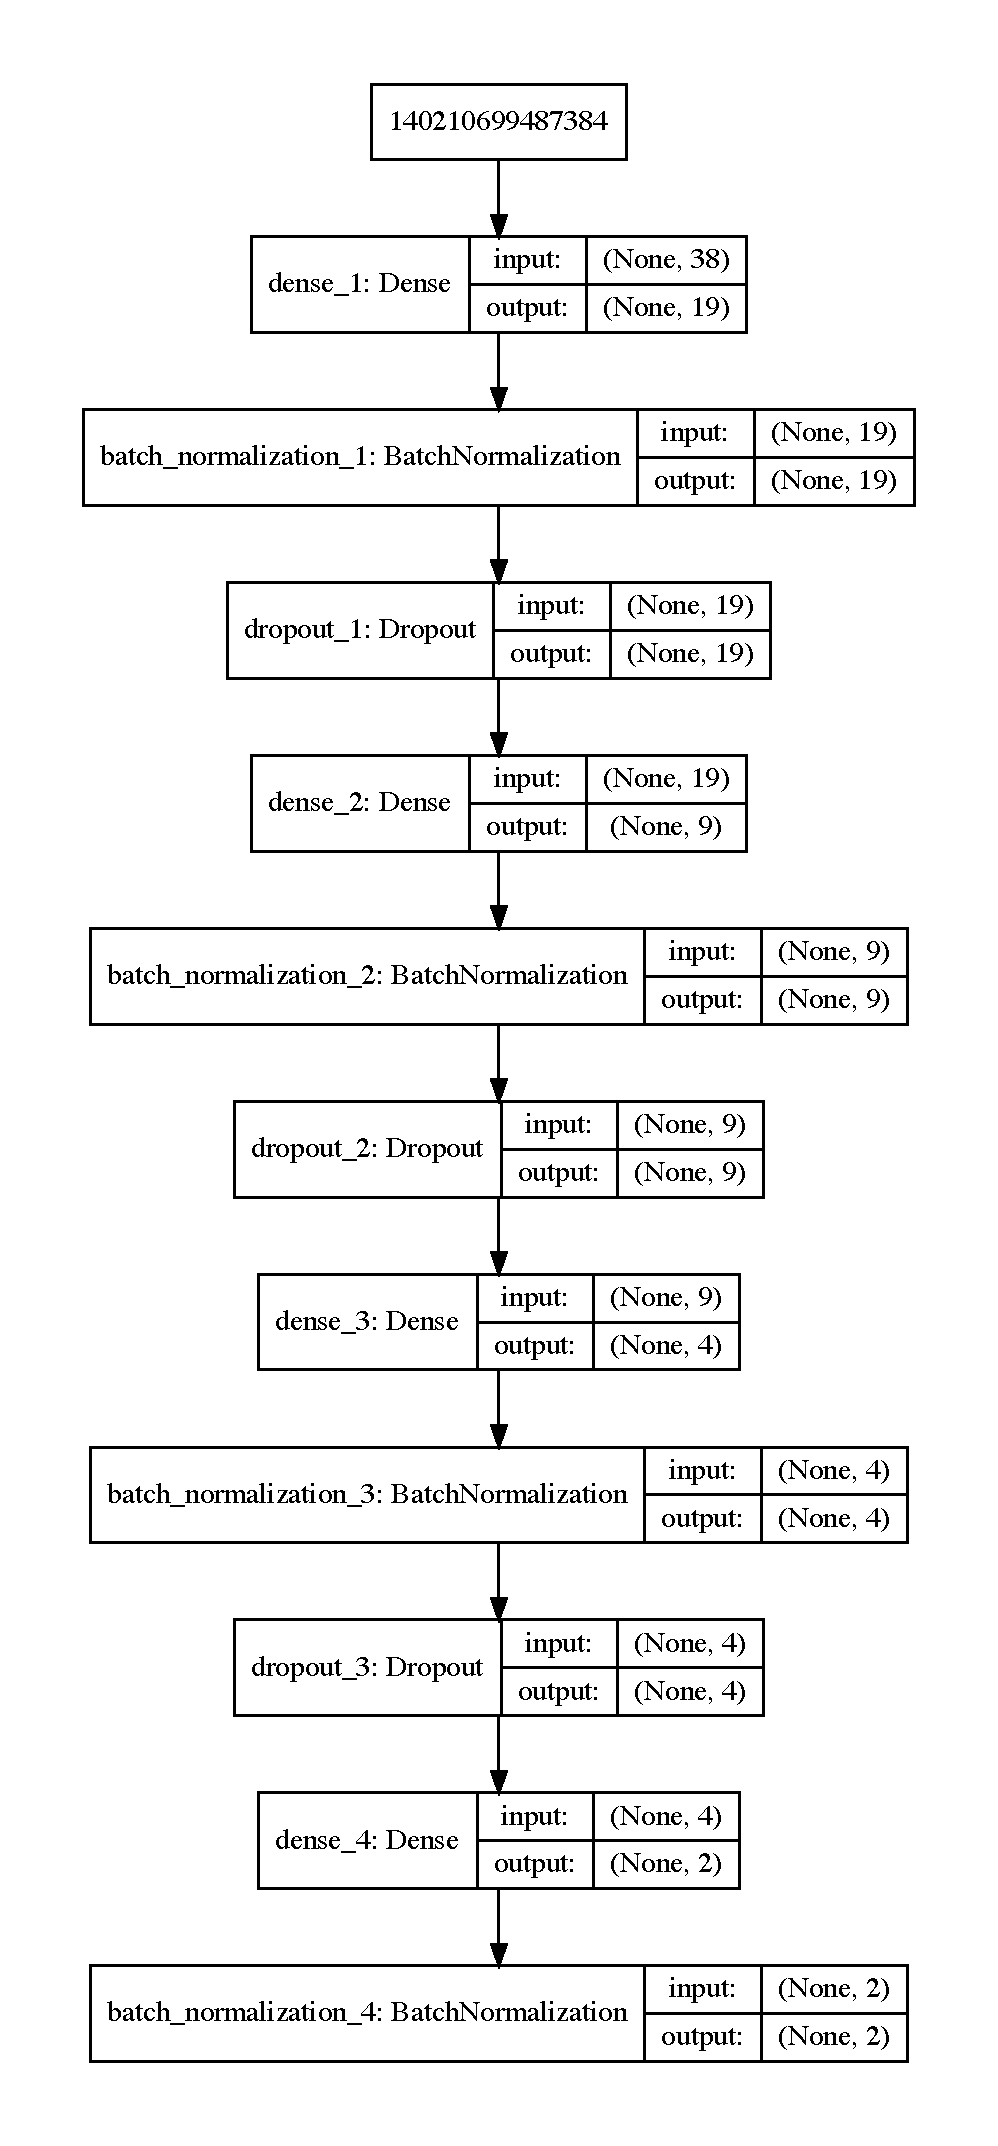
\includegraphics[scale=0.6]{./images/model_ae.pdf}
      \caption{\label{fig_ae}Autoencoder Architecture. }
\end{figure}

\begin{figure}[ht!]
  \centering
  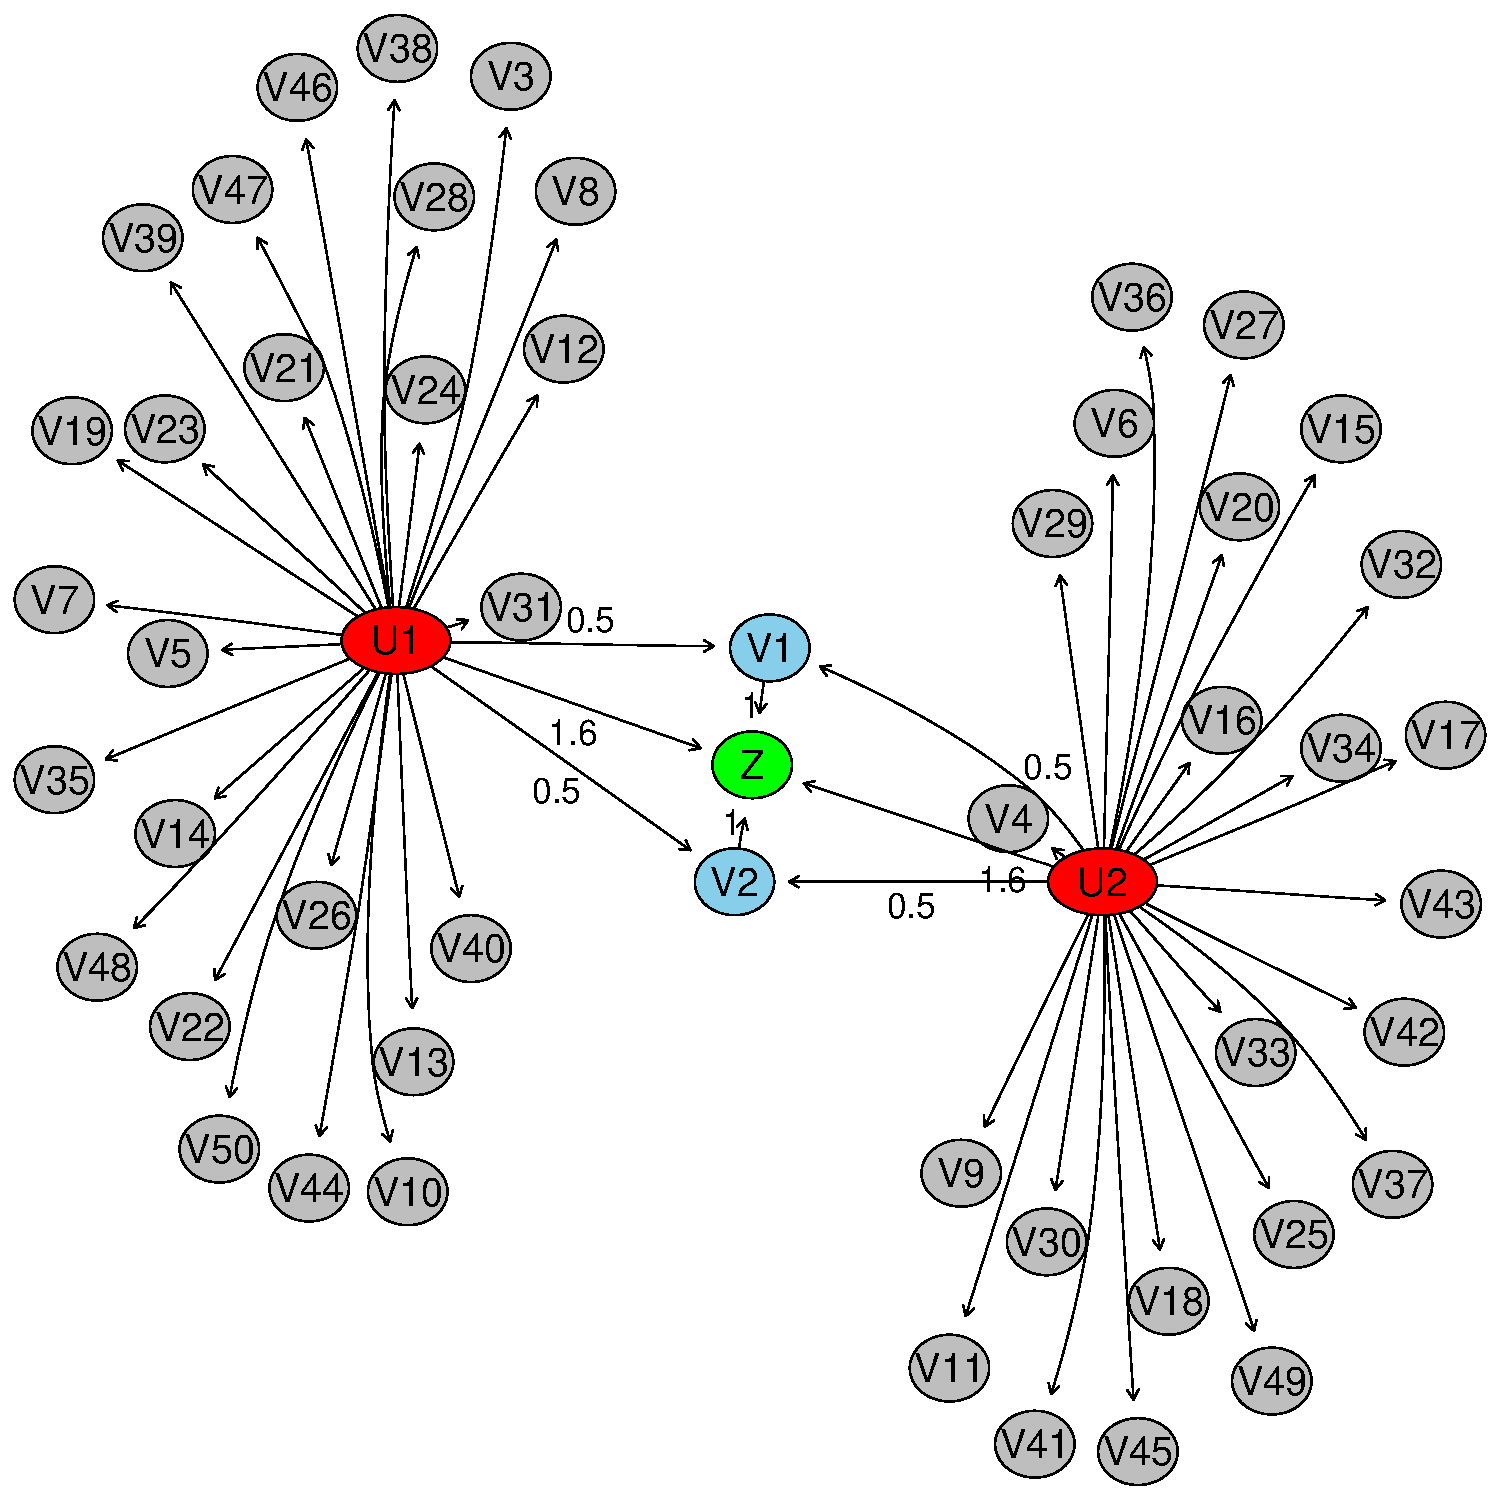
\includegraphics[width=\linewidth]{./images/true_network.pdf}
      \caption{\label{fig_network_true}True network. }
\end{figure}
\begin{figure}[ht!]
  \centering
  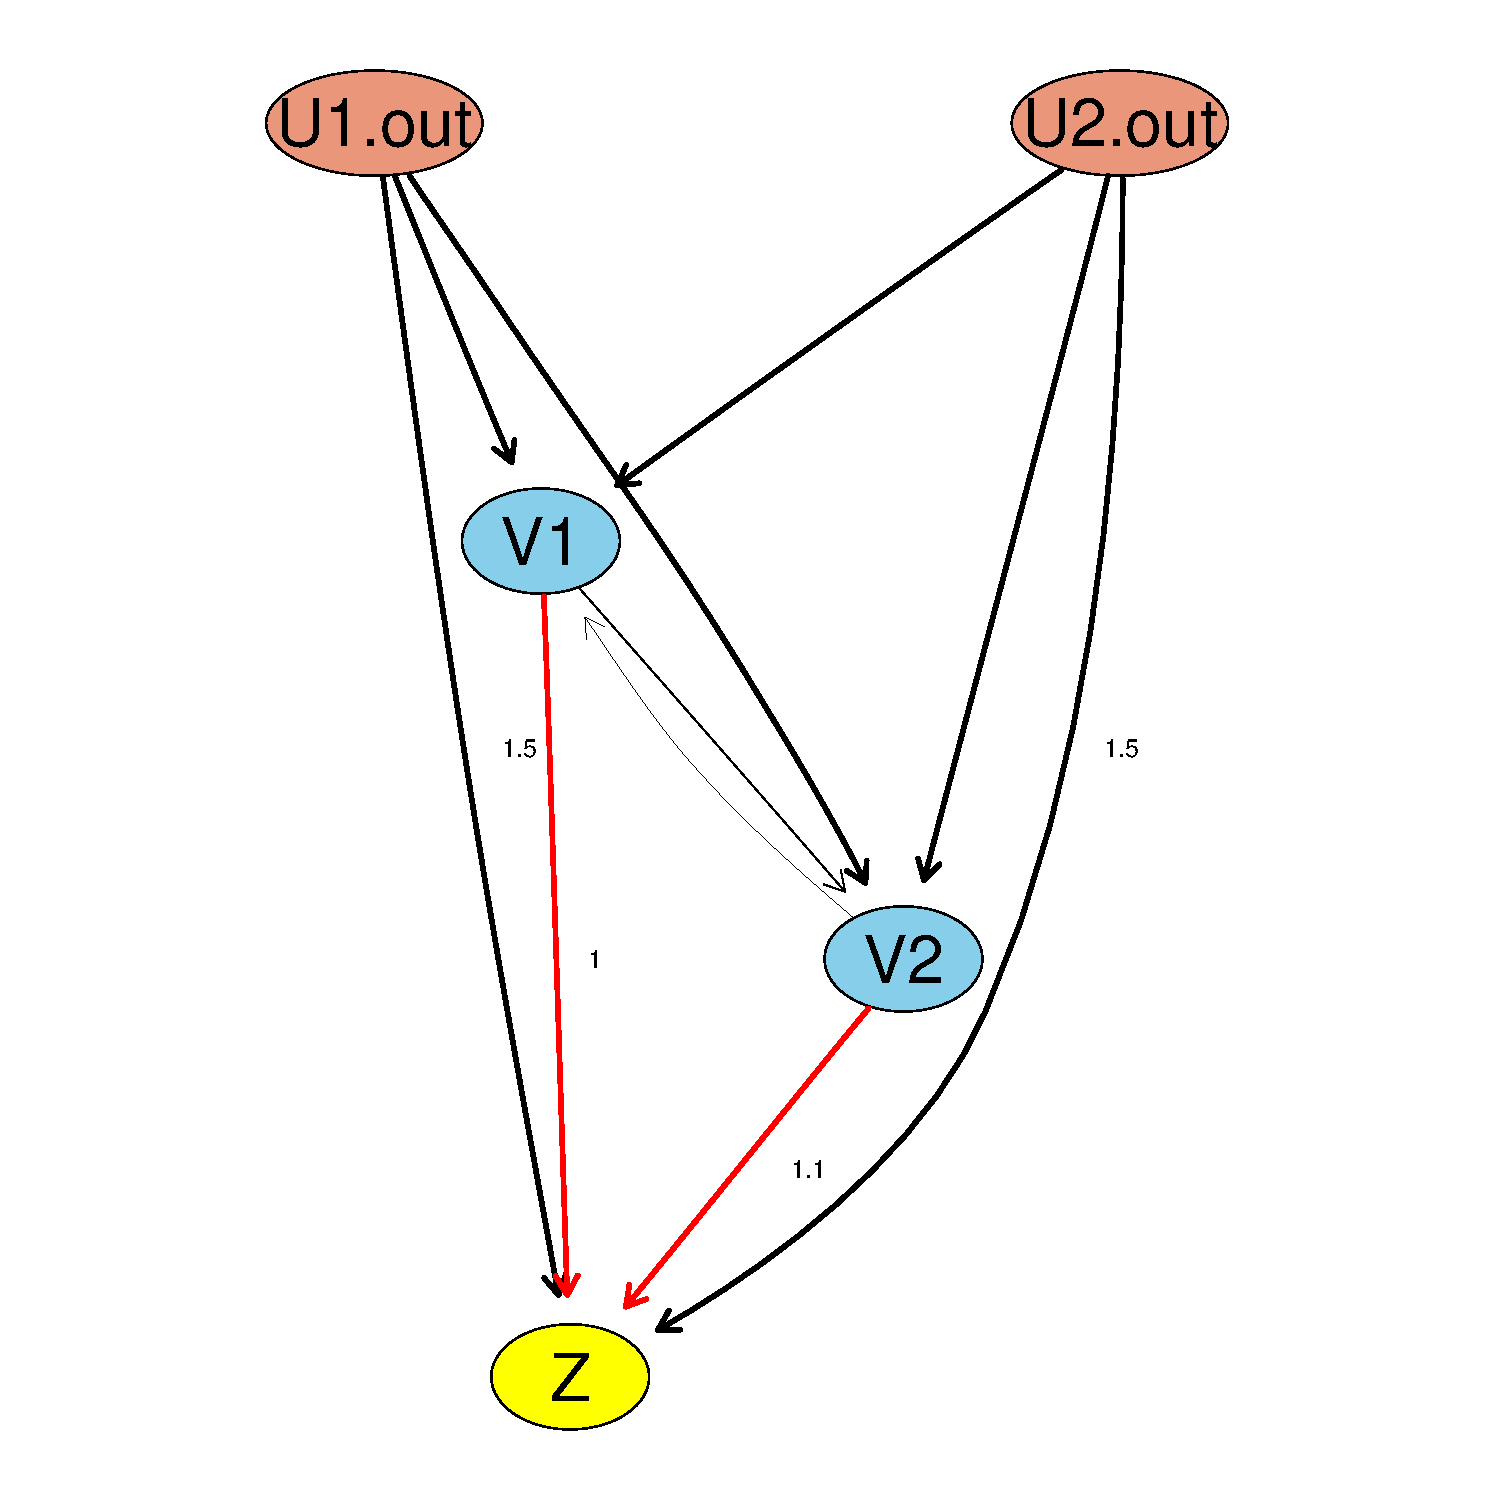
\includegraphics[width=\linewidth]{./images/estimated_network_fulldata.pdf}
      \caption{\label{fig_network_full}Infered network with complete dataset. }
\end{figure}

\begin{figure}[ht!]
  \centering
  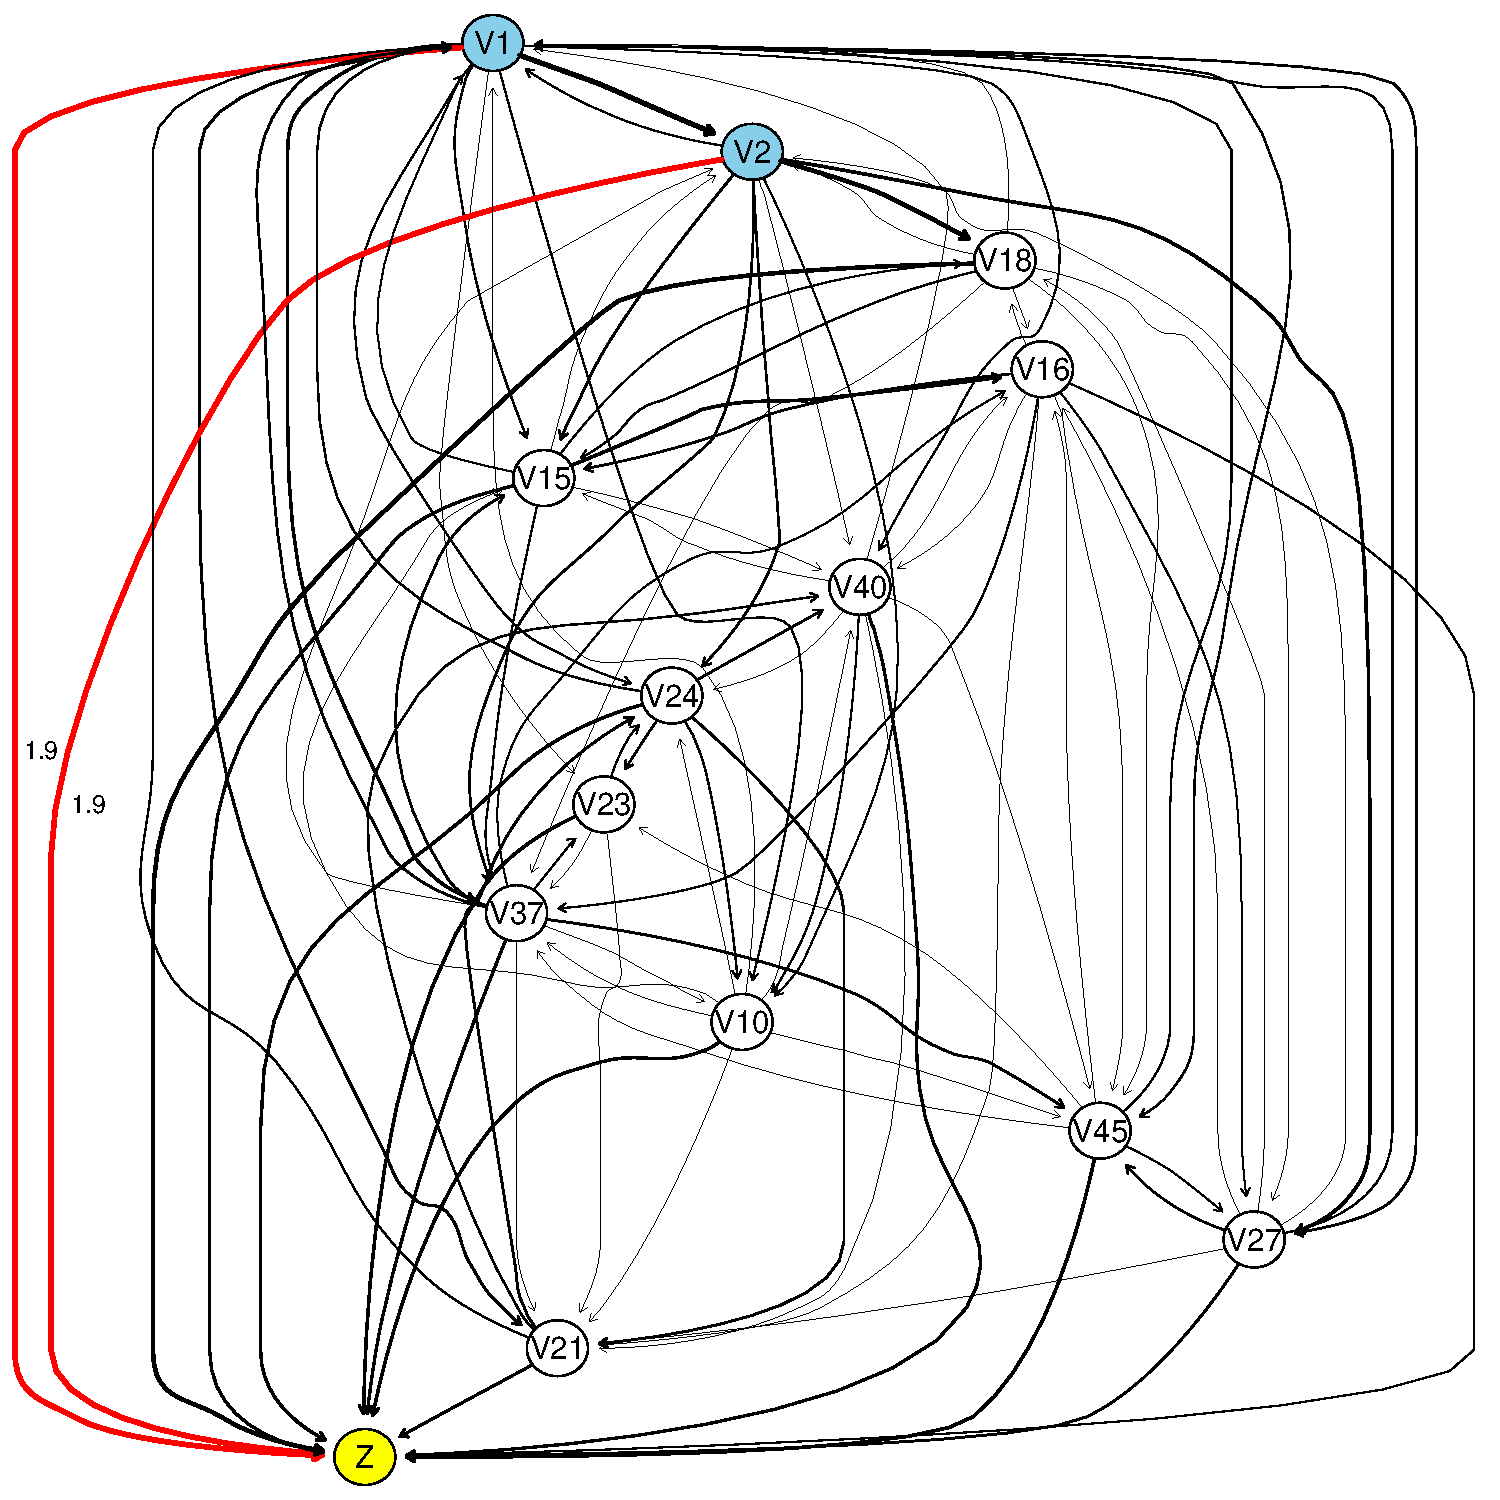
\includegraphics[width=\linewidth]{./images/estimated_network_missingdata.pdf}
      \caption{\label{fig_network_miss}Infered network when $U_1$ and
      $U_2$ are unobserved. }
\end{figure}


\begin{figure}[ht!]
  \centering
  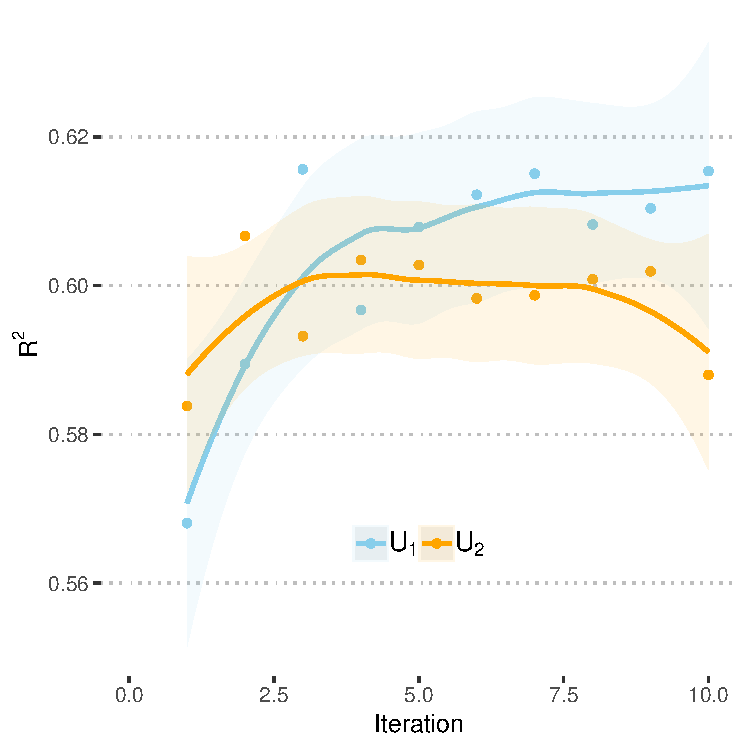
\includegraphics[width=\linewidth]{./images/fig_paper_r2lat.pdf}
      \caption{\label{fig_latvar_r2} $R^2$ in the prediction of the latent variable from the selected principal components}
\end{figure}

\begin{figure}[ht!]
  \centering
  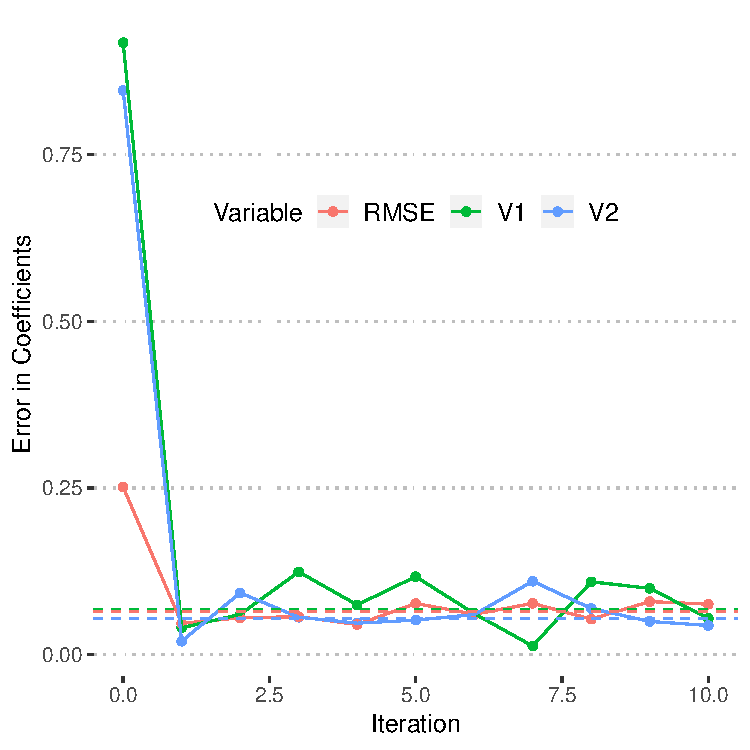
\includegraphics[width=\linewidth]{./images/fig_paper_errors.pdf}
      \caption{\label{fig_coef_rmse} Error in coefficients as a function of the iterations.}
\end{figure}


\begin{figure}[ht!]
  \centering
  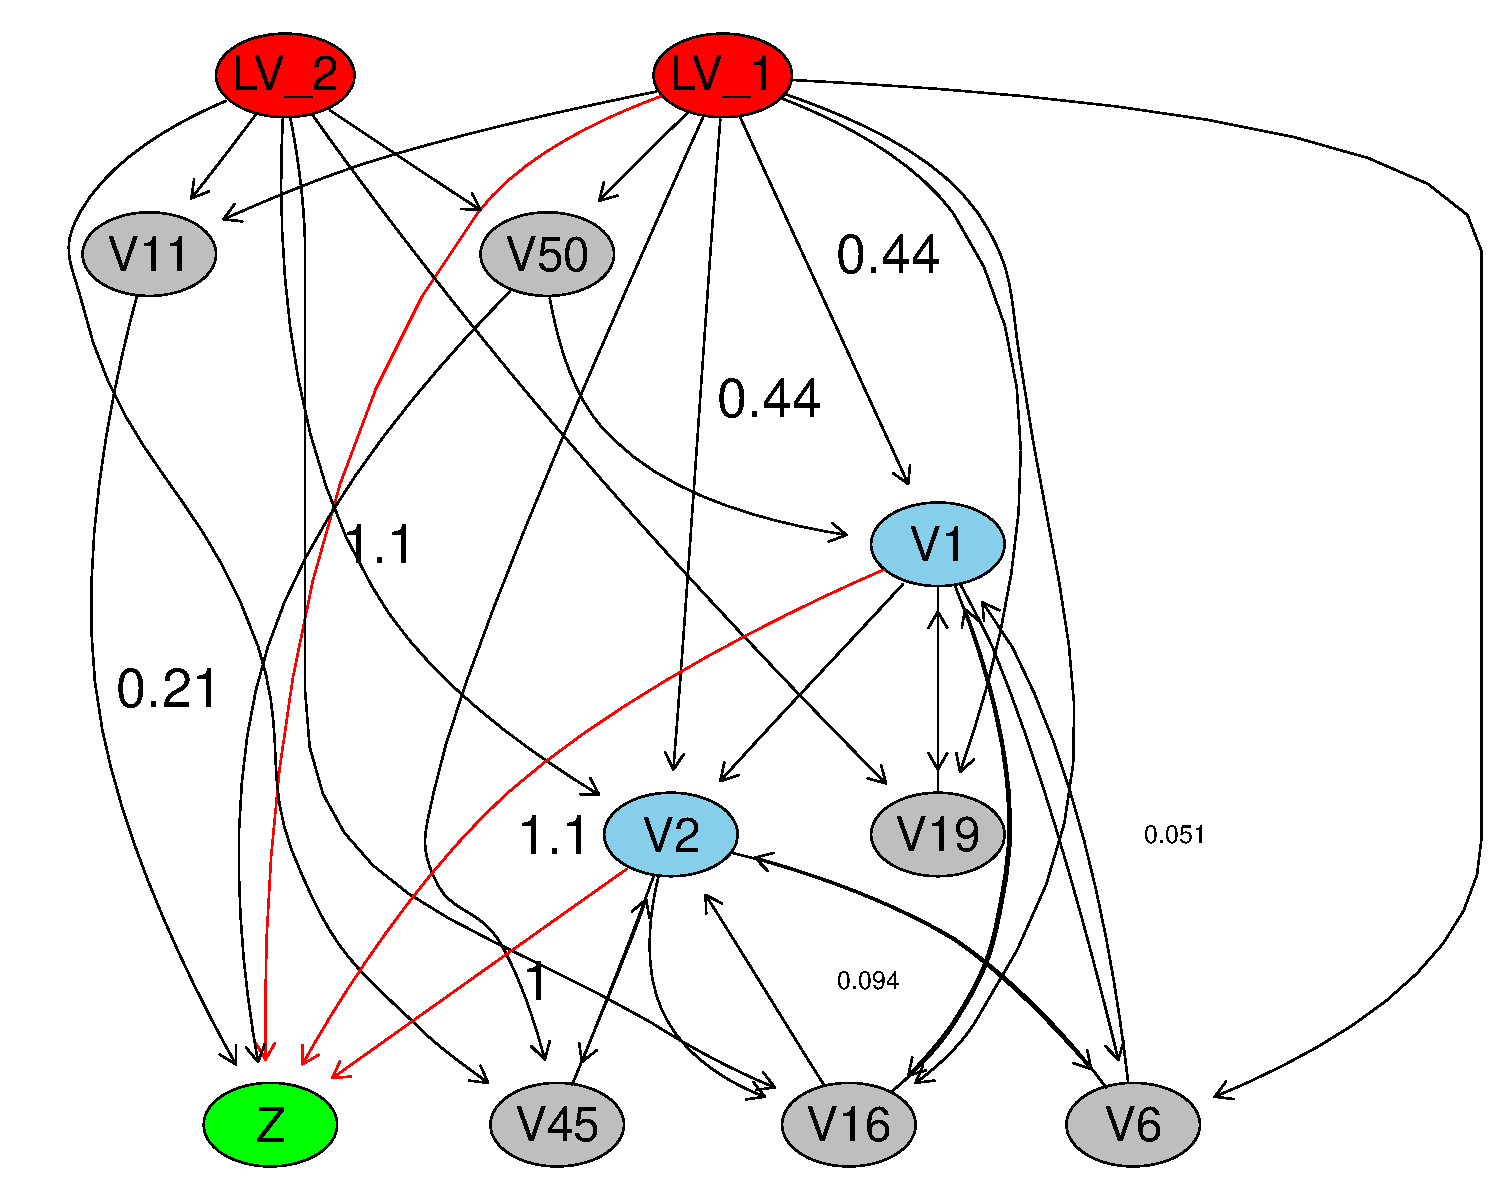
\includegraphics[width=\linewidth]{./images/estimated_network_infered.pdf}
      \caption{\label{fig_network_learn}Infered network at the last
      iteration of algorithm. }
\end{figure}

\begin{figure}[ht!]
  \centering
  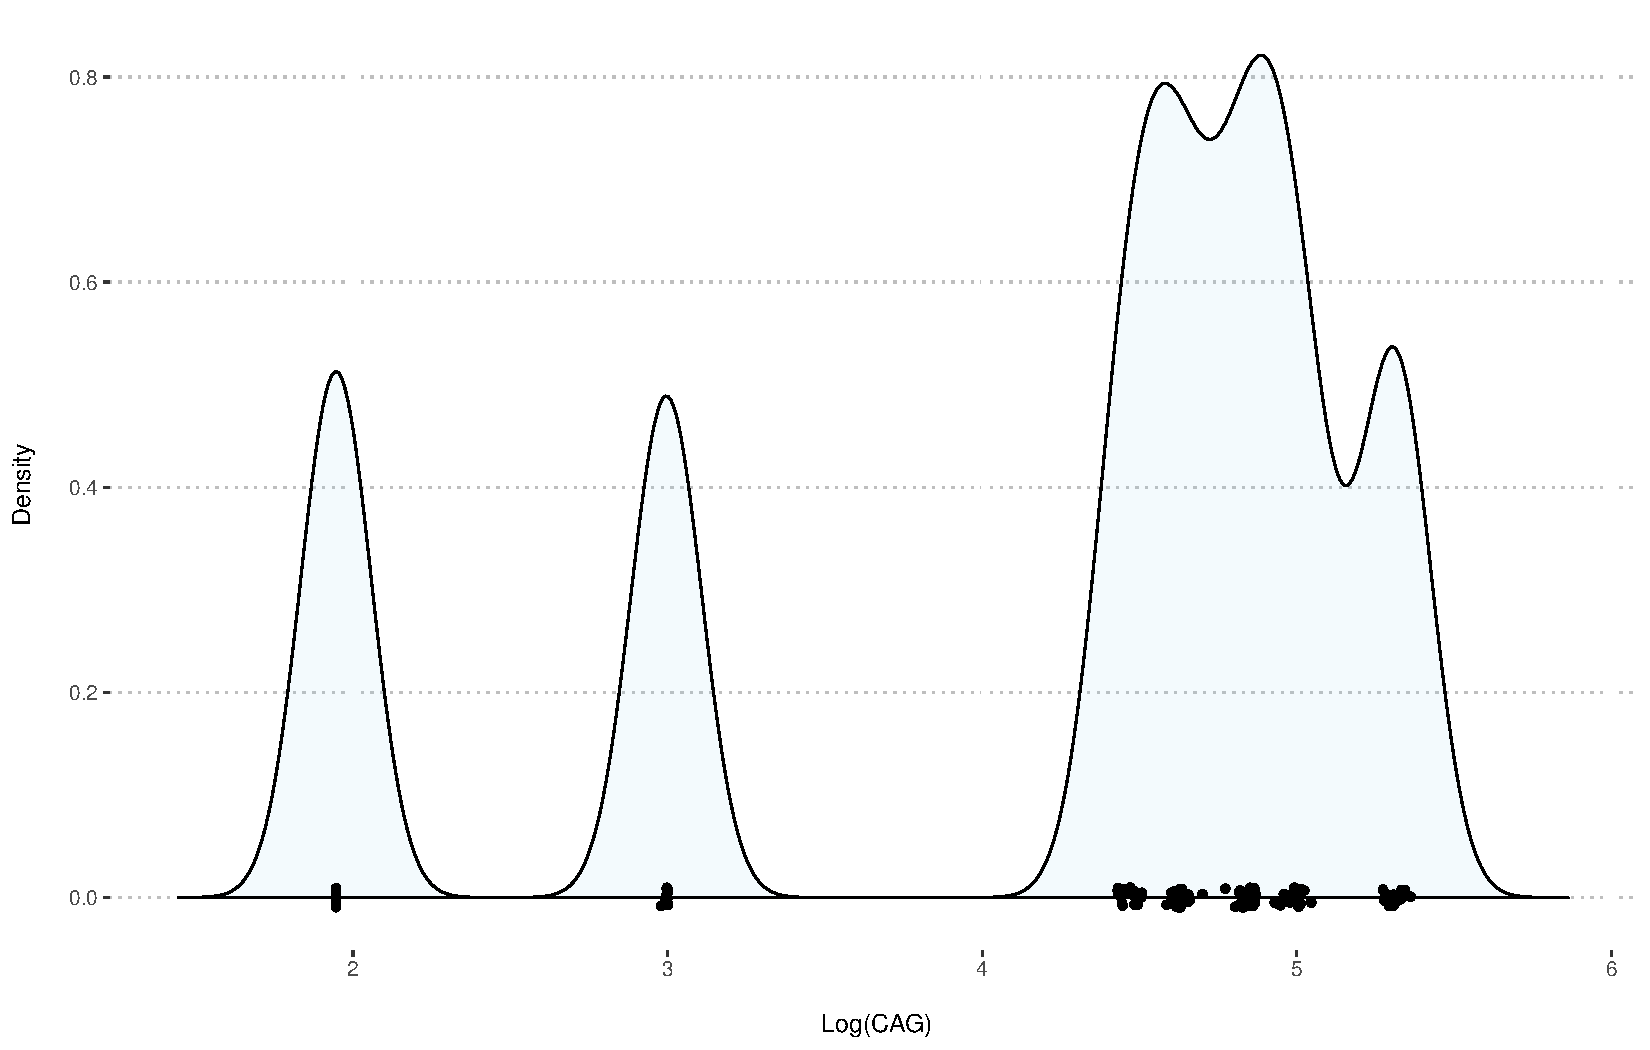
\includegraphics[width=\linewidth]{./images/cagPlots.pdf}
      \caption{\label{fig_cag_density} Density distribution of CAG. }
\end{figure}

\clearpage
\section{Additional Algorithms}
In this section we include additional algorithms

\begin{algorithm}%[H]
 \caption{Assesment Of Inference Of Latent CAG Repeat Length}
 \label{alg_cag}
\begin{algorithmic}
\STATE {\bfseries Data:} The CAG dataset, with CAG repeat length withheld
\STATE \textbf{Result:} Latent space predictive of CAG in training data and code to predict out of sample
 \FOR{fold $in$ 5 folds} 
  \STATE Train on 4/5 of the data
  \STATE Learn latent variables (linear, autoencoder methods)
  \STATE Predict out of sample
 \ENDFOR
 \STATE Concatenate all out-of-sample predictions across folds
 \STATE Assess $R^{2}$ for linear and autoencoder methods
\end{algorithmic}
\end{algorithm}

\clearpage
\section{Additional Examples}
\small
\bibliography{LatentVars}
\bibliographystyle{icml2020}

\end{document}
